
%% Basierend auf einer TeXnicCenter-Vorlage von Mark Müller
%%%%%%%%%%%%%%%%%%%%%%%%%%%%%%%%%%%%%%%%%%%%%%%%%%%%%%%%%%%%%%%%%%%%%%%

% Wählen Sie die Optionen aus, indem Sie % vor der Option entfernen  
% Dokumentation des KOMA-Script-Packets: scrguide

%%%%%%%%%%%%%%%%%%%%%%%%%%%%%%%%%%%%%%%%%%%%%%%%%%%%%%%%%%%%%%%%%%%%%%%
%% Optionen zum Layout des Artikels                                  %%
%%%%%%%%%%%%%%%%%%%%%%%%%%%%%%%%%%%%%%%%%%%%%%%%%%%%%%%%%%%%%%%%%%%%%%%
\documentclass[%
%a4paper,							% alle weiteren Papierformat einstellbar
%landscape,						% Querformat
10pt,								  % Schriftgröße (12pt, 11pt (Standard))
BCOR0.8cm,						% Bindekorrektur, bspw. 1 cm
%DIV=calc,						% führt die Satzspiegelberechnung neu aus
%											  s. scrguide 2.4
%twoside,							% Doppelseiten
%twocolumn,						% zweispaltiger Satz
parskip=half*,				% Absatzformatierung s. scrguide 3.1
%headsepline,					% Trennline zum Seitenkopf	
%footsepline,					% Trennline zum Seitenfuß
%titlepage,						% Titelei auf eigener Seite
%normalheadings,			% Überschriften etwas kleiner (smallheadings)
%idxtotoc,						% Index im Inhaltsverzeichnis
%liststotoc,					% Abb.- und Tab.verzeichnis im Inhalt
%bibtotoc,						% Literaturverzeichnis im Inhalt
%abstracton,					% Überschrift über der Zusammenfassung an	
%leqno,   						% Nummerierung von Gleichungen links
%fleqn,								% Ausgabe von Gleichungen linksbündig
%draft								% überlangen Zeilen in Ausgabe gekennzeichnet
]
{scrartcl}

%\pagestyle{empty}		% keine Kopf und Fußzeile (k. Seitenzahl)
%\pagestyle{plain}	  % lebender Kolumnentitel  

%% Deutsche Anpassungen %%%%%%%%%%%%%%%%%%%%%%%%%%%%%%%%%%%%%%%%%%%%%%%
\usepackage[ngerman]{babel}
\usepackage[T1]{fontenc}
\usepackage[latin1]{inputenc}
\usepackage{lmodern} %Type1-Schriftart für nicht-englische Texte

%% Packages für Grafiken, Abbildungen & Farbe %%%%%%%%%%%%%%%%%%%%%%%%%
\usepackage{graphicx} %%Zum Laden von Grafiken
\usepackage{amsmath} %%Mathepaket
\usepackage{tabularx}
%\usepackage{geometry}
\usepackage{subfigure} %%Teilabbildungen in einer Abbildung
%\usepackage{tikz} %%Vektorgrafiken aus LaTeX heraus erstellen
\usepackage{color}
\usepackage{colortbl}
	\definecolor{hellgrau}{rgb}{0.95,0.95,0.95}
\usepackage{listings}
\usepackage{algorithmic}

%% PDF-Optionen %%%%%%%%%%%%%%%%%%%%%%%%%%%%%%%%%%%%%%%%%%%%%%%%%%%%%%%
%\usepackage[
%	pdftitle={},
%	pdfsubject={},
%	pdfauthor={},
%	linktocpage=true,
%	pagecolor=darkblue,
%	pdfkeywords={}
%]{hyperref}


%% Bibliographiestil %%%%%%%%%%%%%%%%%%%%%%%%%%%%%%%%%%%%%%%%%%%%%%%%%%
%\usepackage{natbib}

\begin{document}
%\pagestyle{empty} %%Keine Kopf-/Fusszeilen auf den ersten Seiten.

%%%%%%%%%%%%%%%%%%%%%%%%%%%%%%%%%%%%%%%%%%%%%%%%%%%%%%%%%%%%%%%%%%%%%%%
%% Ihr Artikel                                                       %%
%%%%%%%%%%%%%%%%%%%%%%%%%%%%%%%%%%%%%%%%%%%%%%%%%%%%%%%%%%%%%%%%%%%%%%%

%% eigene Titelseitengestaltung %%%%%%%%%%%%%%%%%%%%%%%%%%%%%%%%%%%%%%%    
%\begin{titlepage}
%% Basierend auf einer TeXnicCenter-Vorlage von Tino Weinkauf.
%%%%%%%%%%%%%%%%%%%%%%%%%%%%%%%%%%%%%%%%%%%%%%%%%%%%%%%%%%%%%%

%%%%%%%%%%%%%%%%%%%%%%%%%%%%%%%%%%%%%%%%%%%%%%%%%%%%%%%%%%%%%
%% Deckblatt
%%%%%%%%%%%%%%%%%%%%%%%%%%%%%%%%%%%%%%%%%%%%%%%%%%%%%%%%%%%%%
%%
%% ACHTUNG: Sie benötigen ein Hauptdokument, um diese Datei
%%          benutzen zu können. Verwenden Sie im Hauptdokument
%%          den Befehl "\input{dateiname}", um diese
%%          Datei einzubinden.
%%
\begin{titlepage}

\begin{flushleft}
	
\includegraphics{Bilder/UniLogo.jpg}
\end{flushleft}

\begin{center}
\vspace{1cm}
\huge
	\textsc{Messungen und Vergleich von Virtualisierungsumgebungen\\}
\LARGE
\vspace{0,5cm}
	\textsc{Entwicklung eines Testframeworks\\}
\vspace{2cm}
\large
	eingereicht von\\
	\textbf{Christoph Steindl (0706052)}\\
\vspace{2cm}
\huge
	\textsc{Bachelorarbeit\\}
\vspace{2cm}
\large
	Studienrichtung: Medieninformatik\\
	Fakult�t f�r Informatik der Universit�t Wien\\
\vspace{2cm}
	Betreuer:\\
	Prof. Dr. K. Tutschku\\
	Bakk. (FH) A. Rafetseder, MSc

\end{center}
\end{titlepage}
%\end{titlepage}

%% Angaben zur Standardformatierung des Titels %%%%%%%%%%%%%%%%%%%%%%%%
%\titlehead{Titelkopf }
%\subject{Typisierung}
%\title{Titel}
%\author{Autor}
%\and{Der Name des Co-Autoren}
%\thanks{Fußnote}			% entspr. \footnote im Fließtext
%\date{}							% falls anderes, als das aktuelle gewünscht
%\publishers{Herausgeber}

%% Widmungsseite %%%%%%%%%%%%%%%%%%%%%%%%%%%%%%%%%%%%%%%%%%%%%%%%%%%%%%
%\dedication{Widmung}
%\maketitle 						% Titelei wird erzeugt

%% Zusammenfassung nach Titel, vor Inhaltsverzeichnis %%%%%%%%%%%%%%%%%
\pagestyle{plain}
\pagenumbering{Roman}
\subsection*{Eidesstattliche Erkl�rung}

Ich erkl�re hiermit an Eides Statt, dass ich die vorliegende Arbeit selbst�ndig und ohne Benutzung anderer als der angegebenen Hilfsmittel angefertigt habe; die aus fremden Quellen (einschlie�lich elektronischer Quellen) direkt oder indirekt �bernommenen Gedanken sind ausnahmslos als solche kenntlich gemacht.\\

Wien, 15. November 2011 \hspace{\fill} Christoph Steindl\\

\subsection*{Zusammenfassung}
Im Zuge dieser Arbeit wurde ein Framework implementiert, mit dem man Aussagen �ber die Fairness eines VMM (Virtual Machine Monitor) machen kann. Um dies zu erreichen, werden in mehreren virtuellen Maschinen Belastungstests synchron durchgef�hrt und deren Laufzeiten geloggt. Anhand dieser Zeiten wird versucht herauszufinden, ob gewisse virtuelle Maschinen bevorzugt werden und daher der VMM beziehungsweise dessen Scheduling-Mechanismus fair arbeitet.
\subsection*{Abstract}
Alleine das immer h�ufigere Auftreten des Begriffes "`Cloud Computing"' in Zeitungen, Magazinen und vergleichbaren Medien zeigt, dass der Begriff "`Virtualisierung"' immer pr�senter wird. Diese so genannte "`Cloud"' stellt jedermann virtuelle Ressourcen zur Verf�gung, die er selbst gar nicht besitzt, aber trotzdem verwenden kann. Doch nicht nur in der "`Cloud"' wirt virtuell gearbeitet, denn der Schritt der Virtualisierung beginnt schon viel fr�her, n�mlich zum Beispiel bei seiner eigenen Hardware. Man ist eigentlich fast tagt�glich damit konfrontiert, ohne es zu merken. Doch nur weil etwas virtuell ist, hei�t dies noch lange nicht, dass es keine G�te besitzt und die Qualit�ten der einzelnen virtuellen Services nicht variieren k�nnen. Dies ist der Punkt, wo diese Bachelorarbeit ansetzt. Im Zuge dieser Arbeit wurde ein Framework erstellt, mit dem man Aussagen �ber virtuelle Maschinen, beziehungsweise �ber die Monitore, welche die virtuellen Maschinen steuern, machen kann. Dieses Framework soll zeigen, ob diese Monitore immer fair arbeiten und somit die einzelnen virtuellen Maschinen gleichgestellt sind.

\clearpage

%% Erzeugung von Verzeichnissen %%%%%%%%%%%%%%%%%%%%%%%%%%%%%%%%%%%%%%%
\tableofcontents			% Inhaltsverzeichnis
\clearpage
\listoftables				% Tabellenverzeichnis
\listoffigures				% Abbildungsverzeichnis
\clearpage


%% Der Text %%%%%%%%%%%%%%%%%%%%%%%%%%%%%%%%%%%%%%%%%%%%%%%%%%%%%%%%%%%
\pagenumbering{arabic}
\setcounter{page}{1}
\newpage
\lstset{language=python, 
						basicstyle=\small, 
						tabsize=2,
						showspaces=false,
						showstringspaces=false,
						numbers = left}
\section{Einleitung}
\subsection{Aufgabenstellung}
Das Thema dieser Arbeit "`Messungen und Vergleich von Virtualisierungsumgebungen"' beinhaltet schon in seinem Titel eine der zentralen Komponenten dieser Arbeit, n�mlich den Begriff der "`Virtualisierung"'. In gr��eren Firmen ist es schon g�ngige Praxis nicht mehr f�r jeden Mitarbeiter einen eigenen vollwertigen PC zu kaufen, sondern man steigt um auf so genannte "`Slim Clients"'. Diese Clients dienen als Schnittstelle zwischen dem Mitarbeiter der Firma und der virtuellen Instanz eines Betriebssystems, welches auf einem Server l�uft. Da man einen geringeren finanziellen Aufwand mit virtuellen Umgebungen, Instanzen und Systemen hat, ist diese Praxis auch im Privatbereich verbreitet.
Doch muss nat�rlich auch hier garantiert werden, dass die Virtualisierung von beliebigen Komponenten fair abl�uft, also dass es keine Bevorzugung von einzelnen Komponenten gegen�ber anderen gibt. Auch wenn man diese Fairness nat�rlich auch auf einer sehr hardwarenahen Ebene testen k�nnte, wird in der folgenden Arbeit vor allem auf virtuelle Maschinen, also Betriebssysteme, welche auf virtuellen Hardware-Komponenten basieren, eingegangen. Um diese Fairness gew�hrleisten zu k�nnen, gilt es ein Framework zu erstellen, mit dem Aussagen �ber die Gleichbereichtigung einzelner virtueller Maschinen gemacht werden k�nnen. Neben der Implementierung des Frameworks ist auch das Ausf�hren von Tests und deren Analyse Teil dieser Arbeit. Eine zus�tzliche Anforderung ist Portabilit�t zu erreichen, sodass das Framework m�glichst auf allen unterschiedlichen Konfigurationen von Hardware und Software eingesetzt werden kann und der Aufwand des Testers/Users, der die Tests durchf�hren will, minimiert werden kann. M�glichst gro�e Teile des Frameworks sollen daher automatisch ablaufen k�nnen.

\newpage
\section{Virtuelle Maschinen}
Dass die Verwendung von virtuellen Maschinen nicht nur ein kurzfristiges Ph�nomen ist, zeigt wahrscheinlich am allerdeutlichsten, dass gro�e IT-Firmen jeweils ihre eigenen Programme zur Erstellung ebendieser implementiert haben, beziehungsweise jeweils eigene Hypervisor zur Verf�gung stellen. Aber auch die Open-Source-Community hat mit dem Projekt \textit{Xen Hypervisor} das Thema der Virtualisierung aufgegriffen. Eine Auflistung einiger Virtualisierungsprojekte von unterschiedlichen Firmen ist in Tabelle \ref{tab:Hypervisor} zu finden. Auch ein Gro�unternehmen wie \textit{IBM} setzt, auch wenn nicht eigens eine Software implementiert wird, auf Virtualisierung und zwar mit einer engen Integration anderer Virtualisierungsumgebungen \cite{IBMSystems.2005}.
\begin{table}[tbp]
	\centering
		\begin{tabular}{ c | c }
			Hypervisor & zugeh�rige Firmen \\
			\hline
			Oracle VM VirtualBox \cite{VBox} & Oracle\\
			Windows Virtual PC \cite{Mic} & Microsoft\\
			Xen Hypervisor \cite{Xen}& Citrix Systems, Inc.\\
			VMware \cite{VMware}& VMware, Inc.
		\end{tabular}
	\caption{Liste unterschiedlicher Hypervisor}
	\label{tab:Hypervisor}
\end{table}
\subsection{Virtualisierung} 
\subsubsection{Vorteile von Virtualisierung}
Nun stellt sich die Frage, wieso man diesen Schritt zur Virtualisierung von Hardware �berhaupt machen soll. \cite{Menasce.2005} gibt m�gliche Antworten und z�hlt mehrere Gr�nde auf:
\begin{itemize}
	\item Sicherheit: Durch die Abkapslung der einzelnen virtuellen Komponenten von der echten Hardware und zwischen den einzelnen Betriebssysteme f�llt ein Angriff auf die Sicherheit eines Systems nicht sehr gravierend aus. Kommt es zu einem Angriff auf eines der virtuellen Systeme, bleiben andere Systeme, die auf der gleichen Hardware laufen, unbetroffen.
	\item Zuverl�ssigkeit und Verf�gbarkeit: Kommt es zu einem Software-Fehler innerhalb einer VM so ist das System rundherum nicht betroffen und die �brigen virtuellen Instanzen stehen nach wie vor zur Verf�gung. Dar�ber hinaus k�nnen virtuelle Maschinen auch in Echtzeit neu organisiert oder auf andere Maschinen migiriert werden ("`Live Migration"'). Die virtuelle Maschine ist w�hrend einer Migration f�r andere Prozesse w�hrend der ganzen Dauer verf�gbar \cite{Clark.2005}.
	\item Kostenaufwand: Wie bereits erw�hnt kommt mit Virtualisierung meist auch eine Ersparnis an Kosten, durch geringeren Anschaffungsaufwand, vor allem in gr��eren Unternehmen.
	\item Anpassung bei Belastungs�nderungen: Braucht ein Benutzer aus einem gewissen Grund kurzfristig mehr Ressourcen, so k�nnen ihm diese ohne Hardware zu ver�ndern zur Verf�gung gestellt werden. Voraussetzung f�r dieses Szenario ist nat�rlich, dass die Anforderungen des Benutzers nicht �ber denen der zugrunde liegenden Hardware sind.
	\item Belastungs�nderung: Wird die Belastung f�r ein System zu gro�, k�nnen einzelne virtuelle Maschinen auf andere Systeme migriert werden, um die Last unter diesen Systemen aufzuteilen.
	\item Alte Applikationen: Durch Generieren einer VM ist es immer m�glich das richtige Betriebssystem f�r diverse Applikationen zu w�hlen. Dies bedeutet, dass trotz einer m�glichen Portierung auf ein neues System eine alte Applikation nach wie vor in der virtuellen Maschine ausgef�hrt werden kann. 
\end{itemize}

\subsubsection{Nachteile von Virtualisierung}
Doch Virtualisierung bringt auch Nachteile mit sich. \cite{Sahoo.2010} zeigt einige Schwachstellen von virtuellen Systemen auf:
\begin{itemize}
	\item Overhead: Der Aufwand eine virtuelle Maschine zu betreiben ist gr��er, als w�rde man nur ein natives System verwenden. Man muss die Hardwarekomponenten des Systems mehrfach belasten, was einen Verfall der Performance mit sich bringt. Ziel der Entwicklung in der Virtualisierung muss es sein, dass der Performance-Unterschied zwischen virtuellem und physischem System minimiert wird.
	\item Schwachstellen/Stabilit�t: Die virtuelle Maschine ist nat�rlich abh�ngig von der physischen Hardware. Kommt es hier zu einem Fehler, so kann die virtuelle Maschine davon ebenfalls betroffen sein. Die Hardwarekomponenten, die auch unter gr��erer Last stehen, m�ssen abgesichert werden. Ein Fehler in der Hardware kann gleich mehrere Systeme zum Stillstand bringen.
	\item Konfigurationsschnittstelle: Die Schnittstelle zur Konfiguration (VMM) ist sehr eng mit den virtuellen Maschinen verbunden. Kommt es zu unerwarteten Zwischenf�llen, sind auch hier gleich mehrere Systeme betroffen. Mit dem VMM gibt es eine Komponente mehr, die gegen Fehler gesch�tzt werden muss, damit das System reibungslos l�uft.
\end{itemize}

\subsubsection{Scheduling}
Jeder Hypervisor einer virtuellen Maschine muss eine Zugriffsregelung (Scheduling) betreiben, mit dem er Ressourcen den einzelnen virtuellen Maschinen zuweisen kann. Dieses Scheduling-Verfahren kann in der Norm zweierlei Qualit�tskriterien erf�llen:
\begin{itemize}
	\item Maximale Auslastung: Oberstes Ziel ist es, dass soviel Durchsatz auf den einzelnen Hardwarekomponenten wie m�glich erzeugt wird. Dies bedeutet, dass beispielsweise die CPU immer ausgelastet sein sollte, auch wenn nicht immer alle Instanzen einer virtuellen Maschine gleich behandelt werden.
	\item Maximale Fairness: Hier sollen alle Instanzen gleich behandelt werden. Es kann in diesem Fall auch dazu kommen, dass gewisse Komponenten Leerlaufzeiten haben, obwohl eigentlich Auftr�ge f�r diese bereit w�ren.
\end{itemize}
Auch wenn hier die Rede von virtuellen Maschinen ist, so kann man obige �berlegung auf jederlei Schedulingmechanismus �bertragen.
\paragraph{Xen-Scheduling} Bei genannten propriet�ren Virtualisierungsprodukten ist es schwierig, dass man Informationen �ber das Scheduling erh�lt. Allerdings hat man beim Open-Source-Projekt des Xen Hypervisors mehr Chancen.
Beim Scheduling-Verfahren von Xen handelt sich um ein so genanntes "`Credit-Scheduling"'. Dies bedeutet, dass jede virtuelle CPU eine gewisse Zeit hat, um ihren Task ausf�hren zu k�nnen. Diese Zeitslots werden in regelm��igen Abst�nden neu vergeben und dann ist es die Aufgabe des Schedulers zu schauen, in welchem Status sich eine virtuelle CPU befindet:
\begin{itemize}
	\item $credit>0$: Es sind noch Zeitressourcen �brig und der Zustand ist UNDER.
	\item $credit\leq0$: Alle Zeitressourcen wurden aufgebraucht und der Zustand ist OVER.
\end{itemize}
Nun werden vom Scheduler die Prozesse von den virtuellen CPUs zuerst gew�hlt, deren Zust�nde auf UNDER sind, welche von den Prozessen gefolgt werden, wo der Zustand OVER ist.
In Sonderf�llen k�nnen die virtuellen CPUs auch auf den Zustand BOOST gesetzt werden, womit sie anderen vorgezogen werden.


\subsection{Aufbau einer virtuellen Maschine}
Um eine virtuelle Maschine einrichten zu k�nnen, bedarf es meherer Komponenten:
\begin{itemize}
	\item Hardware: Auf den Hardwarekomponenten werden alle Vorg�nge, welche in einer virtuellen Maschine vorgehen, tats�chlich ausgef�hrt.
	\item VMM (Virtual Machine Monitor)/Hypervisor: Der VMM regelt die Kommunikation zwischen der Hardware und den virtuellen Maschinen. Der VMM legt f�r die einzelnen virtuellen Maschinen virtuelle Ressourcen an, welche diese dann verwenden k�nnen. Es wird zumindest zwischen drei Typen an VMM unterschieden \cite{IBMSystems.2005}:
	\begin{itemize}
		\item Type 1: Der VMM wird direkt auf der Hardware betrieben.
		\item Type 2: Der VMM wird innerhalb des existierenden Betriebssystems installiert. Dieses funktioniert weiterhin ohne Einschr�nkungen und die Kommunikation mit der Hardware wird �ber dieses so genannte Host-Betriebssystem geregelt.
		\item Hybrid: \cite{Abramson.2006} und \cite{Weng.2009} erweitern diese Typen und sprechen von einem Hybriden-Ansatz, der aus einem kleinen Hypervisor besteht, welcher nur CPU und Speicher verwaltet, w�hrend I/O von den nativen Treibern eines Service-Betriebssystems geregelt werden.
	\end{itemize}
	\item VM (Virtual Machine): Die VM besteht aus den Komponenten, welche von dem VMM f�r sie angelegt wurden. Diese Komponenten k�nnen ganz unterschiedliche Spezifikationen, als die der "`echten"' Hardware haben, indem sie vom VMM emuliert werden.
	\item Guest-Betriebssystem: Innerhalb der VM muss wiederum zur Kommunikation mit der virtuellen Hardware ein weiteres Betriebssystem installiert werden. Dieses kann beliebig gew�hlt werden, da es vom Host-Betriebssystem vollkommen abgekapselt ist. 
\end{itemize}
Zur Veranschaulichung wird in Abbildung \ref{fig:Xen} der Hypervisor der Xen Virtualisierungsumgebung dargestellt. An der links oben abgekoppelten "`Xen Control Software"', die �ber die Driver-Domain\footnote{Eine Dom�ne die Hardwaretreiber enth�lt, um die Kommunikation von nativen und virtuellen Komponenten zu erm�glichen.} mit dem Hypervisor verbunden ist, kann man erkennen, dass es sich hier um einen Type 1-VMM handelt. Ebenfalls gut erkenntlich ist, dass jede Hardwareressource abgekoppelt von der virtualisierten Hardware arbeitet. Weiters sind drei virtuelle Maschinen abgebildet, welche nur �ber den Hypervisor mit der Hardware kommunizieren k�nnen.
\begin{figure}[ht]
	\centering
		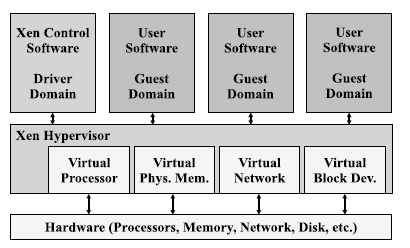
\includegraphics[width=0.8\textwidth]{Bilder/Xen.png}
	\caption{Schematische Darstellung des Xen Hypervisors \cite{Ongaro.2008}.}
	\label{fig:Xen}
\end{figure}

\newpage
\section{Architektur des Frameworks}
\subsection{Design}
Das Design des Frameworks erm�glicht zwei unterschiedliche Kategorien von Tests f�r virtuelle Maschinen:
\begin{itemize}
	\item Sequenziell: Ein Test kann auf einer virtuellen Maschine ausgef�hrt werden. Durch eine Vielzahl an Tests mit unterschiedlichen Konfigurationen kann man einen Schluss �ber die Skalierung des VMM und der virtuellen Mascheinen ziehen. Hier ist wichtig, dass die Tests nacheinander ausgef�hrt werden, damit sie sich untereinander nicht beeintr�chtigen.
	\item Synchron: Es laufen mehrere virtuelle Maschinen, auf welchen gleichzeitig derselbe Test ausgef�hrt wird. Hier stehen die VMs kompetativ zueinander und man kann direkt ablesen, welche VM in einem gewissen Zeitabschnitt eine bessere Performance gezeigt hat. Die Synchronit�t des Systems gelingt nat�rlich immer nur innerhalb gewisser (Rand-)Bedingungen, welche physikalischer Natur sind, weshalb  es schwieriger ist, ein synchrones System zu implementieren.
\end{itemize}
Die Entscheidung wurde f�r ein System, das zumeist im synchronen Betrieb laufen soll, gef�llt, trotzdem wird der sequentielle Betrieb aber unterst�tzt. Um die Prozesse im synchronen Fall m�glichst gleichzeitig ablaufen lassen zu k�nnen, wird eine Instanz implementiert, welche als Monitor fungiert. Die Aufgabe dieser Instanz ist, zu regeln wann welche Kommandos f�r welche Prozesse an die virtuellen Maschinen erteilt werden. Da der Monitor unabh�ngig sein soll, hat sich auch der Platz, wo dieser ausgef�hrt wird, empfohlen. Man kann diesen einfach als Server-Prozess im Host-Betriebssystem ausf�hren und jede einzelne virtuelle Maschine (Client) verbindet sich mit diesem.

Zur Kommunikation zwischen den Instanzen Client und Server wird das verbindungssichere Transport-Control-Protocol (TCP) verwendet.

Weiters wurde Python als Implementierungssprache festgelegt. Grund daf�r war der gute und einfach zu handhabende Socket-Support in Python und au�erdem die einfache Installation im Betriebssystem (bzw. die standardm��ige Vorinstallation in einigen Betriebssystemen). Das Framework soll m�glichst vielseitig, also f�r m�glichst jede Art von VMM, VM und Betriebssystem einsetzbar sein, weshalb Portabilit�t eine wesentliche Rolle f�r das Framework spielt. Daher wurde versucht im Folgenden m�glichst mit der Standardbibliothek aus Python in der Implementierung auszukommen, um den Installationsaufwand m�glichst gering zu halten.

F�r die Leistungsuntersuchung wurde der Fokus auf zwei Gebiete gelegt, auf die n�her eingegangen wird. Einerseits sollte die Zuweisung der Rechenleistung und der Speicherzuteilung, sowie die Performance bei Ein- und Ausgabeoperationen auf der Festplatte genauer unter die Lupe genommen werden, andererseits ist die erreichbare Performance bei hoher Netzlast wichtig. Es wurden Testszenarien in diesen Gebieten entwickelt, welche dann auf den virtuellen Maschinen verwendet werden k�nnen.

\subsubsection{Aufbau der Architektur}
Wie bereits angedeutet, handelt es sich um eine Client-Server-Architektur. Es wird eine Instanz der Klasse \textit{Host} aufgerufen, welche auf einem beliebigen Rechner liegen kann. Innerhalb jeder virtuellen Maschine wird eine Instanz der Klasse \textit{Client} aufgerufen, welche sich mit dem Host verbindet (vgl. Abschnitt \ref{class}). Die Steuerkommunikation findet ausschlie�lich zwischen diesen beiden Instanzen statt. In Abbildung \ref{fig:CD} ist das Framework nochmals grafisch dargestellt. 

\begin{figure}[ht]
	\centering
		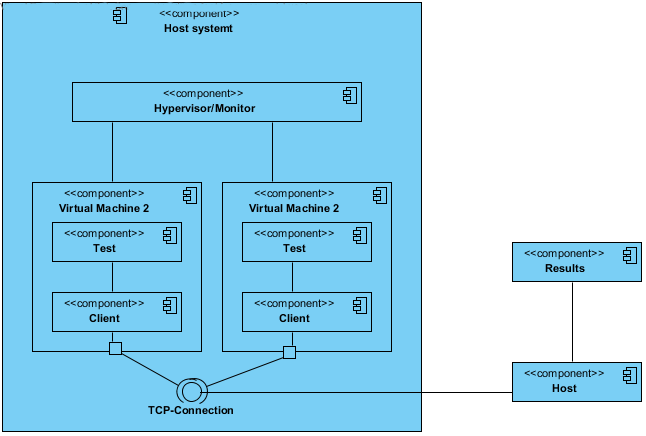
\includegraphics[width=1.00\textwidth]{Bilder/CD.png}
	\caption{Komponentendiagramm des Frameworks mit zwei virtuellen Maschinen}
	\label{fig:CD}
\end{figure}

\subsection{Umsetzung}
Folgend wird auf die endg�ltige Implementation n�her eingegangen. Das Framework reicht von der Abhandlung einzelner Tests bis hin zum Erstellen erster Grafiken und Messwerte, welche die zuvor genannten Tests als Basis nehmen. Die Tests werden in Abschnitt \ref{test} genauer beschrieben.
\subsubsection{Sequenzdiagramm}
Das Sequenzdiagramms in Abbildung \ref{fig:SD} soll den Ablauf des Frameworks genauer veranschaulichen. Nachdem der Tester die Einstellungen f�r die Tests richtig getroffen hat, startet er zuerst das Skript \textit{host.py} mit der Klasse \textit{Host} und danach auf jeder VM das Skript \textit{client.py} mit der Klasse \textit{Client}. Der Client verbindet sich mit dem Host, welcher dann das Ausf�hren des Tests initiiert. Der Test wird im Weiteren durchgef�hrt und eine Evaluation der Messwerte durchgef�hrt.

Das Sequenzdiagramm wurde zur Veranschaulichung im Bereich des Ausf�hren eines Tests ("`4: run test"') vereinfacht. In Wirklichkeit bedarf es hier noch einer Kommunikation zwischen den beiden Instanzen, um zum Beispiel die einzelnen Iterationen synchron zu halten und die Beendigung eines Tests anzuzeigen.
\begin{figure}[ht]
	\centering
		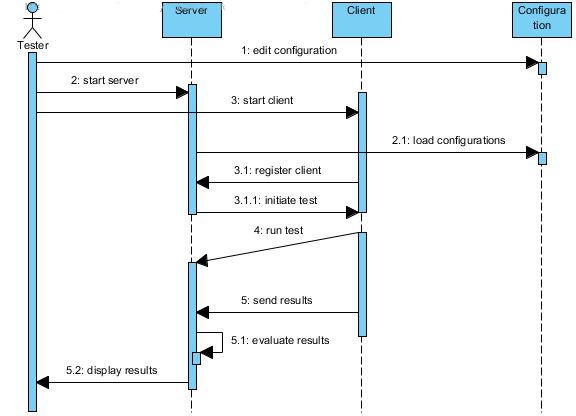
\includegraphics[width=1.00\textwidth]{Bilder/SD.png}
	\caption{Der Ablauf zwischen der Klasse \textit{Host} und einer Klasse \textit{Client} in einem Sequenzdiagramm}
	\label{fig:SD}
\end{figure}


\subsubsection{Klassen-, Datei-, Skriptbeschreibung}\label{class}
Die Umsetzung des Frameworks erfolgt zu einem gro�en Teil in Python-Klassen. Es wurde nur bei einigen Implementierungen (z.B. Evaluierung der Resultate) auf das Klassen-Modell verzichtet, da es nicht n�tig erschien und den Ablauf nicht wesentlich erleichterte. F�r die Speicherung von Daten wurde das CSV-Format verwendet, da dessen Bedienung einfach und intuitiv ist. Abbildung \ref{fig:CD1} verschafft einen �berblick, wo die einzelnen Klassen/Skripte instanziiert werden und zeigt die wesentlichen Assoziationen untereinander auf.
\begin{figure}[ht]
	\centering
		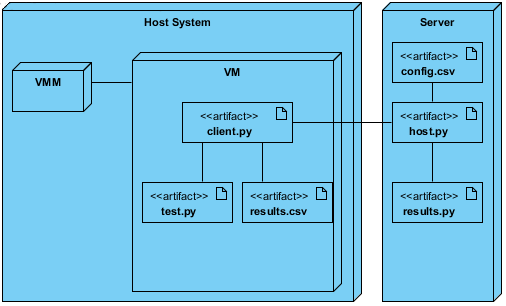
\includegraphics[width=1.00\textwidth]{Bilder/CD1.png}
	\caption{Struktur und Aufteilung der Klassen innerhalb des Frameworks}
	\label{fig:CD1}
\end{figure}
\paragraph{Host}
Die Klasse \textit{Host} ist jene Klasse, welche auf dem Server gestartet werden soll. Sie muss mit folgenden drei Parametern initiiert werden:
\begin{itemize}
	\item Port to listen <int>: Es muss ein gewisser TCP-Port ausgew�hlt und deklariert werden, �ber den eine Verbindung zu dem Server hergestellt werden kann. Die Auswahl dazu sollte im Bereich der frei w�hlbaren Ports liegen und demnach gr��er als 1024 sein.
	\item Number of clients <int>: Hier wird vom Benutzer ausgew�hlt, wieviele Clients (also virtuelle Maschinen) sich mit dem Server verbinden sollten. Bevor besagte Anzahl nicht erreicht ist, werden die Tests nicht gestartet.
	\item Number of iterations <int>: Es wird angegeben, wie oft ein einzelner Testvorgang jeweils wiederholt werden soll.
\end{itemize}
Sobald die Host-Instanz l�uft, wartet sie, dass sich die virtuellen Maschinen verbinden. Ist dies geschehen, beginnt sie eine Liste an Befehlen abzuarbeiten und diese den Clients mitzuteilen. Diese Liste wird von einer Konfigurationsdatei eingelesen und kann folgendes beinhalten:
\begin{itemize}\label{command}
	\item IO: Es wird ein Ein-Ausgabetest gestartet.
	\item Net: Es wird ein Netzwerktest gestartet.
	\item data: Die gesammelten Daten der Clients sollen an den Host geschickt werden.
	\item config: Eine Zusammenstellung der Konfiguration der virtuellen Maschinen (Gr��e Arbeitsspeicher, Prozessor, Betriebssystem) soll an den Host �bermittlet werden.
	\item stopClient: Es wird der Befehl zum Stoppen der Clients an diese �bertragen.
	\item plot: Aus den gesammelten Daten der Clients sollen Graphen erstellt werden.
\end{itemize}
Wird ein Test gestartet, so ist es weiters Aufgabe des Hosts die einzehlnen Iterationen synchron zu halten. Es wird f�r jede zu absolvierende Iteration des Clients ein "`iteration"'-Kommando gesendet, nach dessen Erhalt die Clients damit starten ihren Test durchzuf�hren. Sind alle Iterationen abgehandelt, wird das n�chste Kommando aus der Liste abgearbeitet.
Im Falle von Netzwerktests und der �bermittlung von Daten (config, data) stellt der Server zwischen den Kommandos der Liste den Clients zus�tzlich ein Socket zur Verf�gung, um sich verbinden zu k�nnen.
\paragraph{Client}
Die \textit{Client}-Klasse wird vom User innerhalb der jeweiligen virtuellen Maschine aufgerufen. Dieser Aufruf beinhaltet zwei Parameter:
\begin{itemize}
	\item Port to connect <int>: Hier muss der gleiche Port angegeben werden, wie beim Host, damit sich beide Einheiten �ber diesen Port verbinden k�nnen.
	\item Server IP <String>: Um den Port einer Maschine zuteilen zu k�nnen, muss ebenfalls die IP-Adresse des Hosts angegeben werden. Es ist dabei wichtig die IP des richtigen Netzwerk-Interfaces zu w�hlen, welches mit dem Client verbunden ist. Da der Host potenziell auf derselben Maschine ausgef�hrt wird, wo auch der VMM installiert ist, besitzt sie in diesem Fall zumindest zwei Interfaces, n�mlich ein reelles und ein virtuelles.
\end{itemize}
Die \textit{Client}-Klasse verbindet sich also mit dem Host und erh�lt von diesem ihre Kommandos. Diese sind jeweils zu Tupeln zusammengefasst und haben folgende Struktur: [Kommando, Zusatzinformation]. Diese Kommandos werden ausgelesen und dann in dieser Reihenfolge abgearbeitet. Die Abarbeitung ist entweder das Durchf�hren eines Tests, oder das Senden von Information an den Host.
Die Testergebnisse werden in einer CSV-Datei abgespeichert, welche mit einem Zeitsptempel versehen ist, damit es zu keinem Verlust der Rohdaten kommt, falls es bei der sp�teren �bertragung zu Fehlern kommt.
\paragraph{Const}
\textit{Host}- und \textit{Client}-Klasse k�nnen jeweils eine \textit{Const}-Klasse generieren. Diese Klasse enth�lt keine Methoden, sondern ein W�rterbuch f�r die Kommunikation zwischen Host und Client, weshalb sie vor allem String-Variablen enth�lt, die gewisse Befehle bedeuten. Es k�nnen aber auch Konstanten festgelegt werden, welche sowohl f�r die Server- als auch die Clientseite gelten. Verwendet man diese Klasse \textit{Const} hat dies zum Vorteil, dass man die Konstanten jeweils (seien es numerische Werte oder auch String-Variablen) nur einmal �ndern muss und nicht bei jeder Klasse einzeln.
\paragraph{results.py}
In dem Skript von "`results.py"' werden die gesammelten Werte-Tupel verwertet. Der Host erstellt, wenn in seiner Konfigurationsdatei "`data"' gesetzt ist, eine Datei mit dem Namen "`results.csv"' innerhalb eines Ordners mit dem aktuellen Zeitstempel. Dort sind die Ergebnisse aller Clients nacheinander gespeichert. Es wird dabei immer abgespeichert, um welchen Test es sich handelt und von welchem Client die Daten stammen. Die Datei wird ausgelesen und mit den Werten Graphen erstellt. Um dieses Feature nutzen zu k�nnen m�ssen die Bibliotheken \textit{matplotlib} \cite{mat} und \textit{NumPy} \cite{scipy} installiert sein. Es k�nnen hierbei folgende Formate ausgew�hlt werden.
\begin{itemize}
	\item \textit{scatter:} Bei diesem Format wird die Laufzeit der einzelnen Iterationen f�r alle Clients als Scatter-Plot aufgetragen.
	\item \textit{sum:} Hier wird die Laufzeit der einzelnen Iterationen jeweils summiert und dann wiederum gegen die Iterationen aufgetragen. Dies geschieht wieder f�r alle Clients in einem Plot.
	\item \textit{stats:} Es wird eine Datei mit dem Namen "`stats.csv"' in dem Ordner, welcher von der \textit{Host}-Klasse mit dem Zeitstempel erstellt wurde, erzeugt. In dieser wird f�r jeden Client folgende statistische Information abgespeichert:
	\begin{itemize}
		\item Mean\_Value: Der Mittelwert aller Iterationen
		\item Variance: Die Varianz aller Iterationen
		\item Std\_Variation: Die Standardabweichung berechnet aus der Varianz
		\item Maximum: Der Maximalwert aller Iterationen
		\item Minimum: Der Minimalwert aller Iterationen
		\item Sum: Die Summe aller Werte der Iterationen 
	\end{itemize}
	\item \textit{hist:} Es wird ein Histogramm erzeugt, das die Verteilung aller Clients zeigt.
	\item \textit{scatter90:} Es wird ein Scatterplot erzeugt, bei dem alle Werte, welche zwischen $0.95*max\leq x \leq max$ und $1.05*min\geq x \geq min$ liegen, ignoriert werden. Dies dient dazu um Au�rei�er zu entfernen, die unter Umst�nden f�r das Messergebnis nicht relevant sind.
\end{itemize}
Die Plot-Kommandos sollten in der "`config.csv"' immer als letzte Kommandos gesetzt werden. Weiters ist darauf zu achten, dass die Maschinen unterschiedliche Namen haben (es muss also \verb|socket.gethostname()| jeweils einen unterschiedlichen Wert zur�ckliefern), da es sonst zu einer falschen Zuordnung der Werte kommen kann.
\paragraph{VBox.py}
Dieses Skript dient dazu, um bei der Verwendung von "`Oracle VM VirtualBox"' als VMM, die Abl�ufe automatisieren zu k�nnen. Das Skript ruft nicht nur die Client-Klasse innerhalb der virtuellen Maschine auf, sondern startet auch diese zuvor bziehungsweise beendet diese danach. In einer Schleife geschalten, k�nnen so ohne Zwischeneingabe des Benutzers Tests mit dem Ausf�hren von nur einem Skriptbefehl abgehandelt werden. Um dieses Skript verwenden zu k�nnen ist es notwendig, die folgenden Parameter anzugeben:
\begin{itemize}
	\item Name <String>: Als Unterscheidungsmerkmal zwischen den einzelnen virtuellen Maschinen dient in \textit{VirtualBox} ein Name. Dieser muss beim Aufruf angegeben werden, um die richtige Maschine starten zu k�nnen.
	\item Path <String>: In der Path-Variable muss angegeben werden, wo in Bezug auf das virtuelle Dateisystem der virtuellen Maschine das Arbeitsverzeichnis des Frameworks liegt, damit einerseits von dort die Dateien des Frameworks aufgerufen werden k�nnen und andererseits Daten dorthin gespeichert werden kann.
	\item Port to connect <int>: Analog wie beim Einzelaufruf muss auch hier ein Port angegeben werden. Geschieht dies nicht, so wird ein Standardport (50007) verwendet.
	\item Server IP <String>: Analog wie beim Einzelaufruf muss auch hier eine IP-Adresse angegeben werden. Geschieht dies nicht, so wird die IP-Adresse des Systems, auf dem das Skript gestartet wird herausgefunden und daf�r verwendet.
\end{itemize}
Um dieses Skript einsetzen zu k�nnen ist die Installation der \textit{VirtualBox-SDK} und der \textit{VirtualBox Guest Additions} Voraussetzung. Diese SDK kann jederzeit unter \cite{Igotti.2008} nachinstalliert werden. Die Gasterweiterung f�r VirtualBox ist Bestandteil der Installation.
\paragraph{config.csv}
In der "`config.csv"'-Datei, werden die Prozesse/Tests abgespeichert, welche bei einem Testdurchlauf abgehandelt werden. Aufbauend auf den Kommandos der \textit{Const}-Klasse, werden dort die Kommandos, welche im Abschnitt \ref{command} genauer beschrieben werden, abgespeichert. Der Vorteil des gew�hlten CSV-Formats ist, dass es einerseits mit Tabellenkalukulationsprogrammen, die dieses Format zumeist unterst�tzen, andererseits mit einem einfachen Editor ver�ndert werden kann.
\paragraph{Test}
Die Klasse \textit{Test} ist eine abstrakte Klasse und beschreibt nur die Funktionen und Variablen, welche allen Subtests zur Verf�gung stehen m�ssen. Es wird zum Beispiel allgemein f�r jede Art von Test Membervariablen wie "`start"' (die Startzeit des Tests), "`path"' (den Pfad zum CSV-Dokument mit den Daten), oder ein Socket-Objekt f�r die Kommunikation mit dem Host erzeugt. Um sp�ter ein Kompositum aus den einzelnen Tests zu entwickeln, wurden auch die Funktionen zum Erzeugen von CPU-, HD- und Netzwerklast in dieser Klasse definiert. Der Aufruf f�r diese erfolgt allerdings erst in der Sub-Klasse.
Die Ergebnisse der einzelnen Subtests werden in einer CSV-Datei gespeichert und haben folgende Stuktur, wobei gilt $i=Iteration$:
\begin{lstlisting}
NewTest, <Test type>, <Client name>
Number of i <int>, Duration of i <float>, Starttime of i <float>
.
.
EndTest
\end{lstlisting}

\subsubsection{Implementierte Tests}\label{test}
\paragraph{Mattest}
Beim Mattest geht es darum den/die Prozessorkern(e) mit einer Rekursion m�glichst auszulasten. Dies wird erreicht, indem die Fibonacci-Folge berechnet wird, welche wie folgt definiert ist:
	\[
	f_{n}=f_{n-1}+f_{n-2}
\]
f�r $n\geq2$. Des weiteren gilt $f_{0}=0$ und $f_{1}=1$.
Diese Funktion kann man folgenderma�en in Python rekursiv beschreiben:
\begin{lstlisting}
    def fib(self, n):
        if n <= 0:
            return 0
        elif n == 1:
            return 1
        else:
            return self.fib(n-1) + self.fib(n-2)
\end{lstlisting}
Der Rechenaufwand steigt mit gr��er werdendem $n$ exponentiell und somit auch die Laufzeit auf den einzelnen virtuellen Maschinen.
\paragraph{I-O}
Beim I/O-Test wird eine Datei einer gewissen Gr��e (bei den in Abschnitt \ref{Erg} gezeigten Tests 20MB) ge�ffnet und danach eingelesen. Der eingelesene Inhalt wird sofort danach wieder in ein andere Datei geschrieben. Es entstehen hier gr��ere Lasten am Prozessor und bei der Festplatte. Die Realisierung sieht folgenderma�en aus:
\begin{lstlisting}
    def IO(self):
        o = open('lorem.txt', 'r')
        data = o.read()
        i = open('temp.txt', 'w')
        i.write(str(data))
        o.close()
        i.close()
\end{lstlisting}
\paragraph{SeekAndWrite}
Dieser Test �hnelt dem zuvor genannten I/O-Test. Es wird hier wiederum eine Datei ge�ffnet, welche diesmal wesentlich gr��er dimensioniert (bei den in Abschnitt \ref{Erg} gezeigten Tests 2,5GB) ist. Danach wird nach einem gewissen String-Muster gesucht, welches vom Host bei der jeweiligen Iteration mitgesendet wird. Nun ist es Aufgabe des Tests die Datei zu �ffnen und nach diesem Teilstring zu suchen. Wurde er gefunden, so muss zu dem Index gesprungen werden und der Teilstring von der Datei plus einer gewissen Anzahl an folgenden Zeichen in eine andere tempor�re Datei geschrieben werden.
Der Suchalgorithmus wurde folgenderma�en implementiert.
\begin{lstlisting}
    def seek(self, s):
        o = open('lorem1.txt', 'r')
        
        lastString = ''
        while True:
            currentString = o.read(self.const.chunkSize)
            lastString = lastString + currentString
            index1 = lastString.find(s)
            if index1 > 0:
                index1 = o.tell()+index1-(2*self.const.chunkSize)
                break
            else:
                lastString = currentString
\end{lstlisting}
\paragraph{TCP}
Der TCP-Test ist ein Netwerktest, der das Verhalten des VMM bei vielen Verbindungsversuchen via TCP beschreibt. Nachdem der Client den Befehl zum Start des Tests bekommen hat, wird vom Host ein Socket ge�ffnet. Der Client versucht sich dorthin mit TCP zu verbinden und schickt einen Teststring an den Host. Danach wird die Verbindung wieder abgebaut. Pro Iteration wird dieser Vorgang mehrere Male wiederholt, um auf eine ann�hernd messbare Laufzeit zu kommen. Der zugeh�rige Auszug aus dem Source-Code f�r den Verbindungsaufbau sieht folgenderma�en aus:
\begin{lstlisting}
    def TCP (self, message, serverIP, port):
        s = socket.socket(socket.AF_INET, socket.SOCK_STREAM)
        s.setsockopt(socket.SOL_SOCKET, socket.SO_REUSEADDR, 1)
        s.connect((serverIP, port))
        s.send(message)
        if message == self.const.stop:
            while True:
                data = s.recv(512)
                if data:
                    break
        s.close()
\end{lstlisting}

\newpage
\section{Testf�lle}
\subsection{Allgemeine Beschreibung}
Das Entwickeln der Tests lief prinzipiell in zwei Phasen ab. Zuerst wurde ein entwickelter Test nativ, also im Host-Betriebssystem und nicht in einer VM, getestet. Hier lief in derselben Windows 7-Umgebung sowohl der Host, als auch der Client. In der zweiten Phase wurde das Testframework sp�ter auf eine virtualisierte Testumgebung portiert, um dort ausf�hrlichere Testungen durchf�hren zu k�nnen.

Die Testumgebung f�r die unten angef�hrten Tests besteht aus einem "`AMD Athlon(tm) 64 X2 Dual Core Processor 5000+"', mit 3GB Hauptspeicher. Als Betriebssystem wurde sowohl f�r das Host-System, als auch f�r die VMs die Linux-Distribution \textit{Ubuntu} in der Version 11.04 verwendet. Anzumerken ist ebenso, dass im Host-Betriebssystem eine 64Bit-Variante und in den Guest-Betriebssystemen eine 32Bit-Variante gew�hlt wurde. Als VMM kam \textit{VirtualBox} von der Firma Oracle in der Version 4.1.2 zum Einsatz. Als Testmaschinen wurden bis zu vier durch Klonen baugleiche virtuelle Maschinen verwendet. Diese verf�gten entweder �ber 256MB oder 128MB Arbeitsspeicher und es wurde ihnen eine 10GB-Festplatte von fixer Gr��e zugewiesen. Weiters wurde der Host des Frameworks immer im Host-Betriebssystem ausgef�hrt.

\subsection{Ergebnisse}\label{Erg}
Im folgenden Abschnitt werden Ergebnisse von Tests diskutiert, welche auf der Testumgebung durchgef�hrt wurden. Plots der Ergebnisse sollen einen �berblick �ber das Verhalten des VMM geben. Die Konfigurationen der einzelnen Tests sind in Tabelle \ref{tab:config} nochmals zusammengefasst. Um die Plots �bersichtlicher zu gestalten wurde auf die Legenden innerhalb der einzelnen Bilder verzichtet. Eine Legende, die f�r alle Bilder der Tests gilt, kann man in Abbildung \ref{fig:Legende} finden. Die virtuellen Maschinen sind von $1$ bis $4$ durchnummeriert und sie wurden auch immer in dieser Reihenfolge hochgefahren und der \textit{Client} des Frameworks gestartet.
\subsubsection{TCP}
\textit{Vgl. Abbildung \ref{fig:TCP} auf Seite \pageref{fig:TCP}}

Besonders interessant am TCP-Test ist das sprunghafte Verhalten der einzelnen Iterationen. Besonders gut im Histogramm in Abbildung \ref{fig:TCP2} sieht man, dass die einzelnen Messwerte immer auf vertikalen Linien zu liegen scheinen. Diese entstehen, da das Protokoll ein Standardtimeout hat, welches abgewartet werden muss, falls Pakete nicht �bermittelt werden k�nnen. Das Timeout ist standardm��ig auf drei Sekunden eingestellt, weshalb im Histogramm die Peaks immer wieder um etwa drei Sekunden zeitversetzt auftreten \cite{Seddigh.2001}\cite{Postel.1981}. Zur Fairness muss man sagen, dass diese nicht besonders beeintr�chtigt ist. Die Mittelwerte liegen n�mlich zwischen $\overline{t}_{min} = 14,82s$ und $\overline{t}_{max} = 16,00s$, somit deren maximale Differenz bei $1,18s$, was bei einer Laufzeit von rund $3000s$ eher vernachl�ssigbar erscheint.
\subsubsection{Mattest}
\textit{Vgl. Abbildung \ref{fig:M} auf Seite \pageref{fig:M}}

Betrachtet man diesen Test, so findet man keine au�ergew�hnlichen Ergebnisse vor. Die Werte liegen im Mittel f�r die Maschinen zwischen $\overline{t}_{min} = 33,36s$ und $\overline{t}_{max} = 33,84s$ dementsprechend ist die Varianz und die Standardabweihung klein. Die Standardabweichung schwankt f�r die vier virtuellen Maschinen im Intervall $\sigma_{min} = 0,33s$ und $\sigma_{max} = 0,40s$. Das Histogramm (Abbildung \ref{fig:M1}) verdeutlicht die sehr nahe am Mittelwert liegenden Werte.
\subsubsection{IO}
\textit{Vgl. Abbildung \ref{fig:IO_1} auf Seite \pageref{fig:IO_1}}

\textit{Vgl. Abbildung \ref{fig:IO_2} auf Seite \pageref{fig:IO_2}}

In diesem Test fallen zwei Ph�nomene auf. Einerseits  sind die Laufzeiten bei diesem Test bimodal verteilt. Sowohl mit 256MB (Abbildung \ref{fig:IO1}) als auch mit 128MB (Abbildung \ref{fig:IO2}) Hauptspeichergr��e gibt es im Histogramm jeweils zwei Peaks, wobei einer von diesen jeweils etwa unter $10$ Sekunden ist und der andere jeweils dar�ber. Des weiteren interessant ist auch, dass die Laufzeiten bei 128MB k�rzer sind. Eine Mutma�ung f�r dieses Verhalten ist ein weniger performantes Swap-Verhalten\footnote{Da in Prozessorn�he nur kleine Arbeitsspeicher zur Verf�gung stehen, m�ssen Daten st�ndig neu abgerufen und verschoben werden. Diese werden dann in andere Speichereinheiten verschoben, was man als "`swap"' versteht} im Falle von 256MB Hauptspeicher.
\subsubsection{SeekAndWrite}
\textit{Vgl. Abbildung \ref{fig:S} auf Seite \pageref{fig:S}}

Die deutlich schwankenden Laufzeiten in Abbildung \ref{fig:S1} sind vielleicht dadurch zu erkl�ren, wenn man annimmt, dass die Laufzeiten abh�ngig von der Position in der Datei sind, zu der gesucht werden muss. Also desto sp�ter in der Datei der gesuchte String vorkommt, desto l�nger dauert dies. Da dieser String aber mit einer Zufallszahl bestimmt wird, variieren die Messwerte sehr. Betrachtet man die Ergebnisse in Abbildung \ref{fig:S2}, so f�llt auf, dass die Gesamtlaufzeit summiert �ber alle Iterationen gro�e Unterschiede aufweist. So betr�gt der Unterschied zwischen langsamster und schnellster Laufzeit circa $435$ Sekunden oder $1,4\%$ der Gesamtlaufzeit von rund $30000$ Sekunden.

\begin{table}%
\begin{tabular}{ c |c | c | c | c }
	Testname & \# Clients & Hauptspeicher & Iterationen & Konfiguration \\
	\hline
	TCP-Test & 4 & 256MB & 200 & 5000 Connects/Iteration \\
	MatTest & 4 & 256MB & 1000 & 35 (Rekursionstiefe) \\
	IO-Test & 4 & 128-256MB & 500 & \\
	SeekAndWrite-Test & 4 & 256MB & 200 & \\
\end{tabular}
\caption{Auflistung der Konfigurationen}
\label{tab:config}
\end{table}

\begin{figure}[ht]
	\centering
		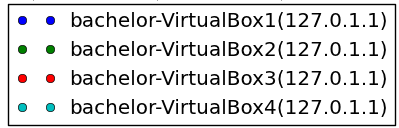
\includegraphics[width=0.7\textwidth]{Bilder/Legende.png}
	\caption{Legende f�r die Plots von Seite \pageref{fig:TCP} bis \pageref{fig:S}}
	\label{fig:Legende}
\end{figure}

\begin{figure}[ht]
	\centering
		\subfigure[Scatterplot eines TCP-Tests]{
			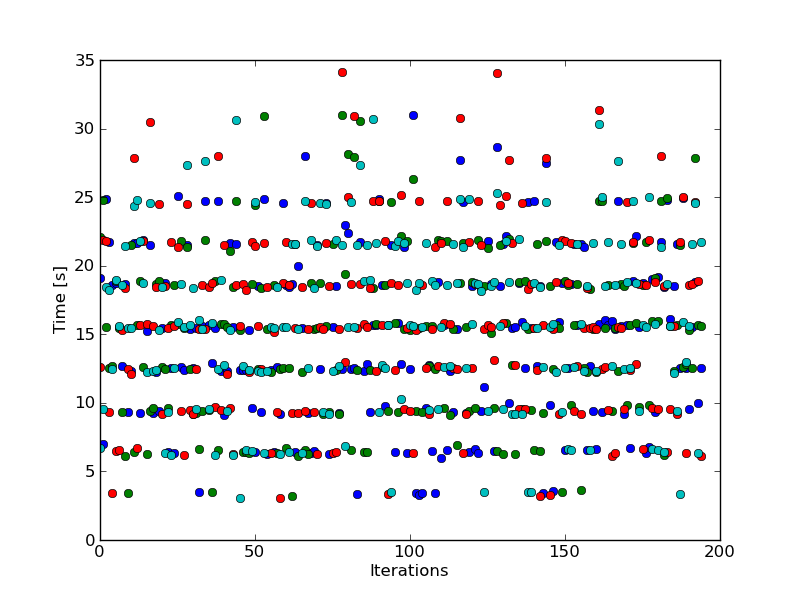
\includegraphics[width=0.85\textwidth]{Bilder/TCP.png}
			\label{fig:TCP1}
		}
	\centering
		\subfigure[Histogramm eines TCP-Tests]{	
			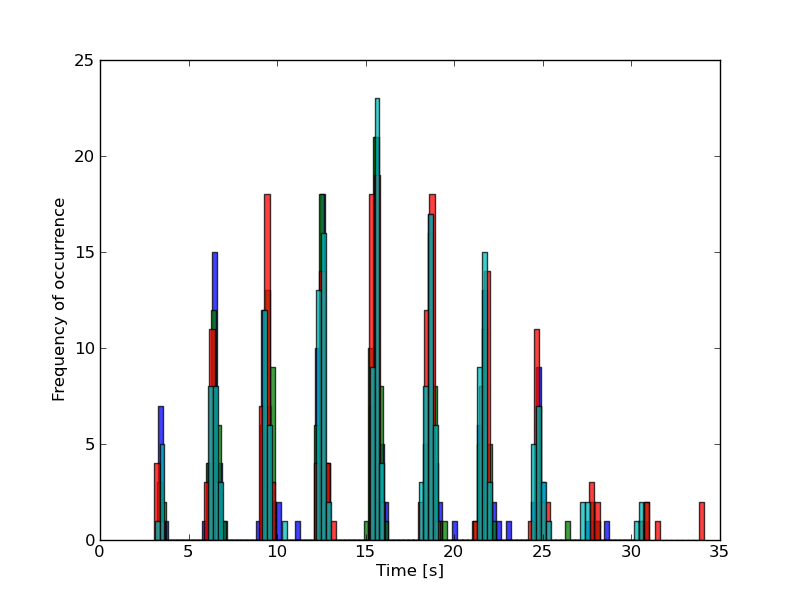
\includegraphics[width=0.85\textwidth]{Bilder/TCPh.png}
			\label{fig:TCP2}
		}
	\caption{Ergebnisse des TCP-Tests}
  \label{fig:TCP}
\end{figure}

\begin{figure}[ht]
	\centering
		\subfigure[Scatterplot eines Mattests]{
			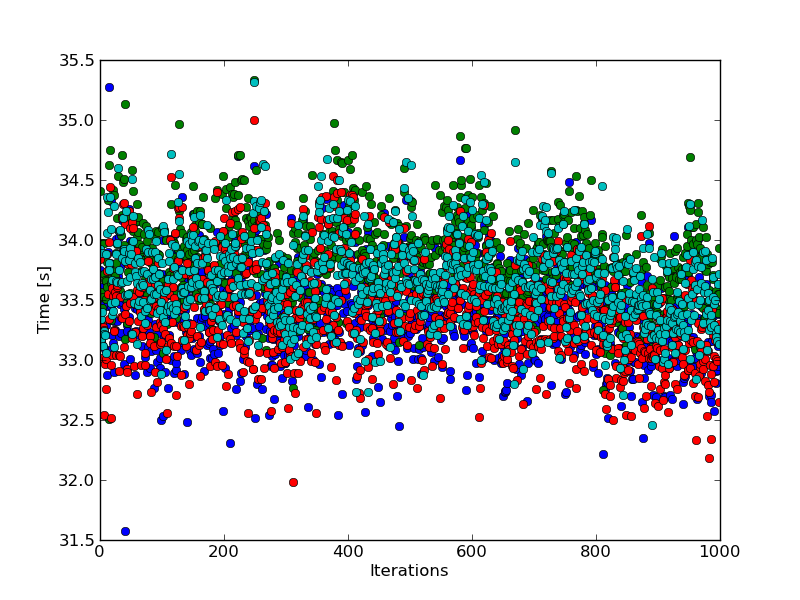
\includegraphics[width=0.85\textwidth]{Bilder/M1.png}
			\label{fig:M1}
		}
	\centering
		\subfigure[Histogramm eines Mattests]{
			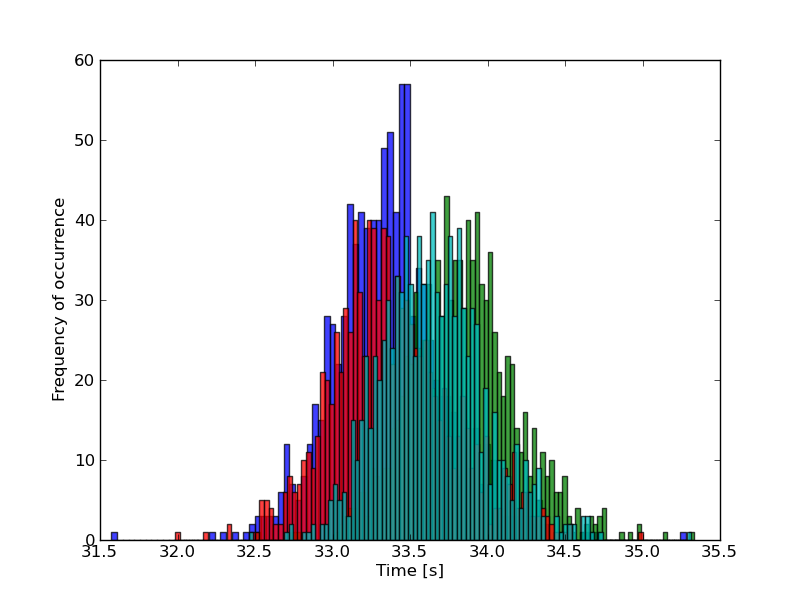
\includegraphics[width=0.85\textwidth]{Bilder/M2.png}
			\label{fig:M2}
		}
	\caption{Ergebnisse des Mattests}
  \label{fig:M}
\end{figure}

\begin{figure}[ht]
	\centering
		\subfigure[Scatterplot eines IO-Tests (256MB Hauptspeicher)]{
			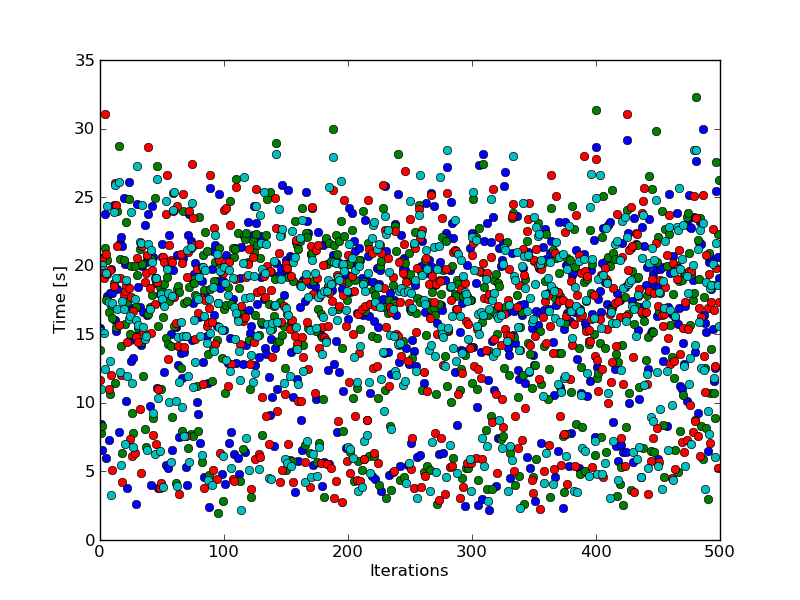
\includegraphics[width=0.85\textwidth]{Bilder/IO1.png}
			\label{fig:IO1}
		}
	\centering
		\subfigure[Histogramm eines IO-Tests (256MB Hauptspeicher)]{
			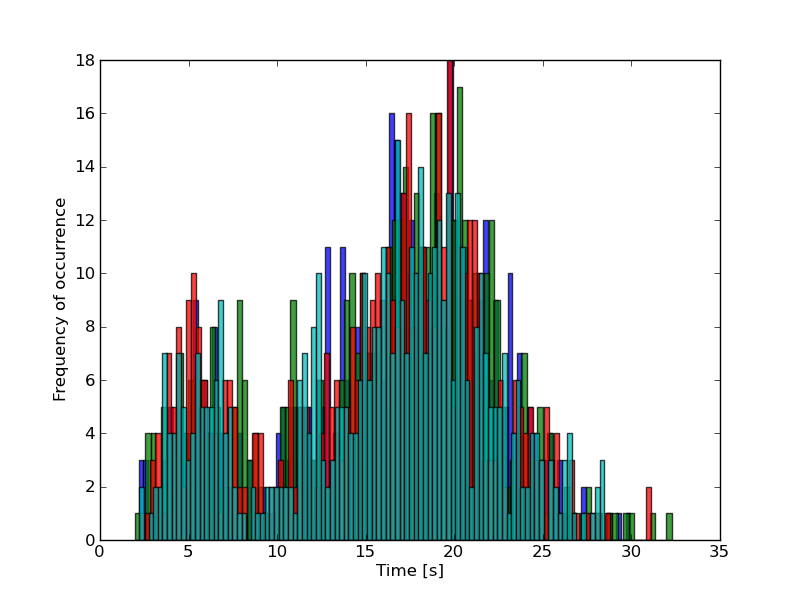
\includegraphics[width=0.85\textwidth]{Bilder/IO3.png}
			\label{fig:IO3}
		}
	\caption{Ergebnisse des IO-Tests bei 256MB Hauptspeicher}
  \label{fig:IO_1}
\end{figure}

\begin{figure}[ht]
	\centering
		\subfigure[Scatterplot eines IO-Tests (128MB Hauptspeicher)]{
			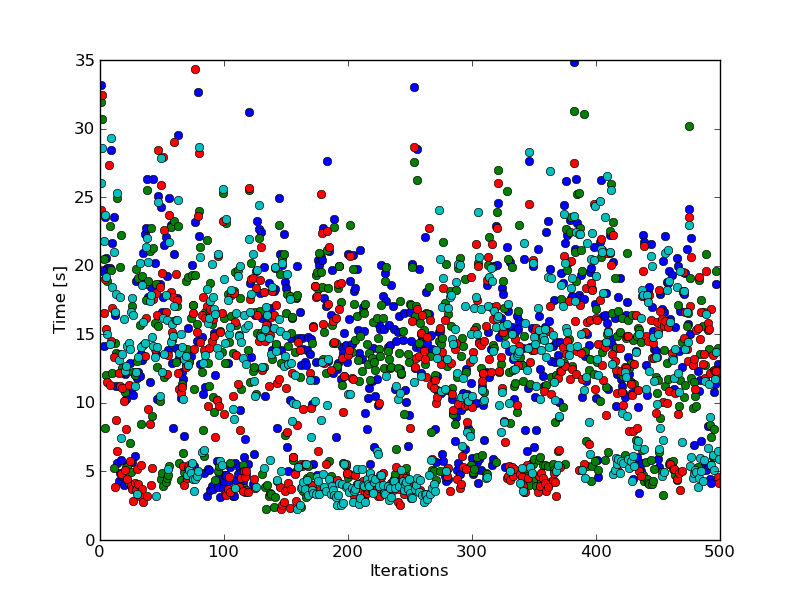
\includegraphics[width=0.85\textwidth]{Bilder/IO2.png}
			\label{fig:IO2}
		}
	\centering
		\subfigure[Histogramm eines IO-Tests (256MB Hauptspeicher)]{
			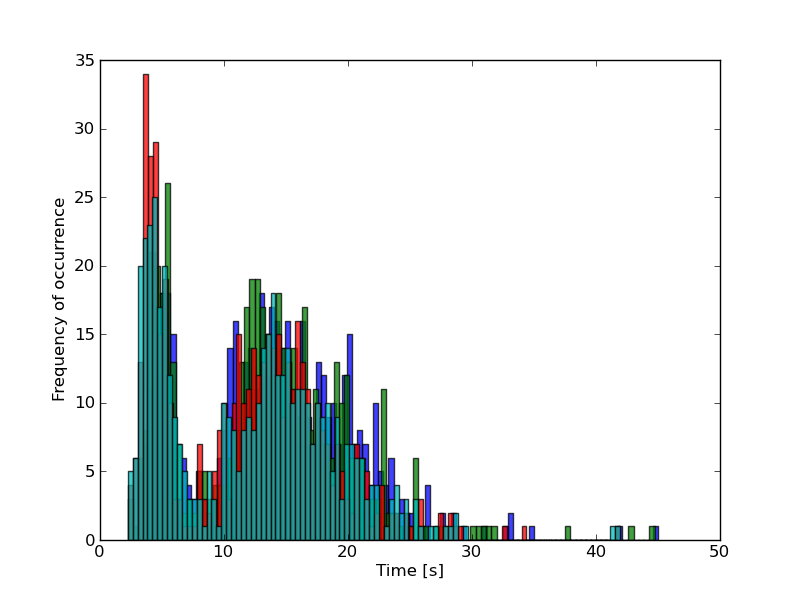
\includegraphics[width=0.85\textwidth]{Bilder/IO4.png}
			\label{fig:IO4}
		}
	\caption{Ergebnisse des IO-Tests bei 128MB Hauptspeicher}
  \label{fig:IO_2}
\end{figure}

\begin{figure}[ht]
	\centering
		\subfigure[Scatterplot eines SeekAndWrite-Tests]{
			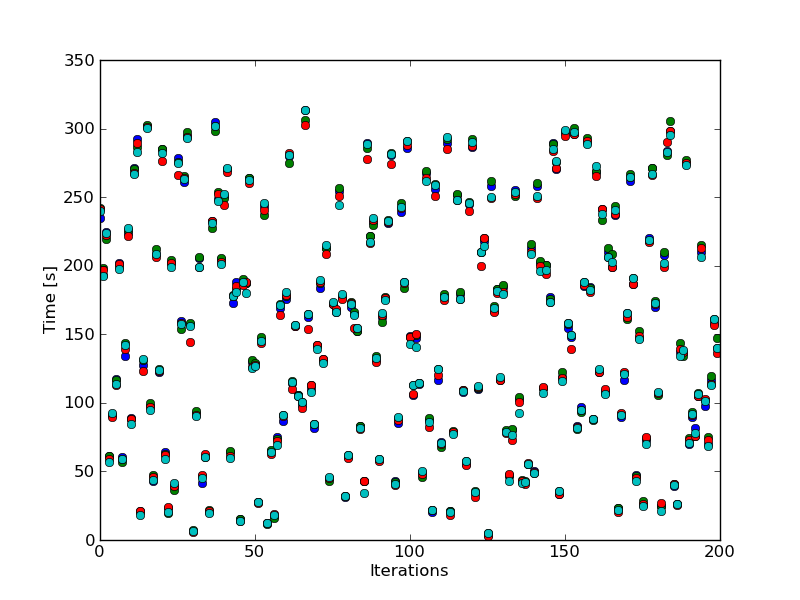
\includegraphics[width=0.85\textwidth]{Bilder/S1.png}
			\label{fig:S1}
		}
	\centering
		\subfigure[Kumulierte Laufzeit eines SeekAndWrite-Tests]{
			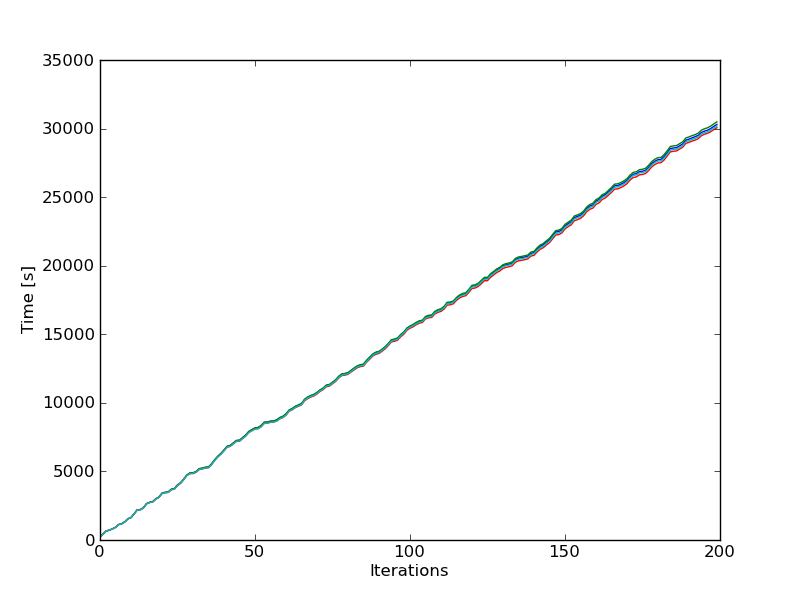
\includegraphics[width=0.85\textwidth]{Bilder/S2.png}
			\label{fig:S2}
		}
	\caption{Ergebnisse des SeekAndWrite-Tests}
  \label{fig:S}
\end{figure}
\clearpage
\newpage
\section{Zukunftspl�ne}
\subsection{Dokumentation}
Um das Framework auch Au�enstehenden zur Verf�gung zu stellen, w�re eine Dokumentation au�erhalb des Codes und dieser Arbeit w�nschenswert. Es w�rde sich hierf�hr wahrscheinlich "`Sphynx - Python Document Generator"' \cite{Sphinx} anbieten, mit dem auch die regul�re Dokumentation von Python gemacht wird.
\subsection{Messkampagnen und Messstrategien}
In den bis jetzt ausgef�hrten Tests wurde die Gr��e des Hauptspeichers variiert. In anderen Messkampagnen k�nnte man genauso andere Hardwarekomponenten skalieren. Man k�nnte beispielsweise genauso die virtuelle Prozessorleistung variieren, beziehungsweise Restriktionen f�r den Netzwerkverkehr setzten, um herauszufinden, ob der VMM in diesen F�llen immer noch fair agiert. Es gibt auch die m�glichkeit zu komplexen Messstrategien, bei denen man mehr als eine Komponente variabel h�lt.
\subsection{Ansteuerung des Hypervisors}
Um das Durchf�hren von den zuvor genannten Messkampagenen und -strategien m�glichst effizient durchsetzten zu k�nnen, w�re das Ansteuern des VMM zwischen einzelnen Tests eine wichtige Komponente. Somit w�re es zum Beispiel m�glich einen Test zu starten und nach dessen Beendigung die Konfiguration mit Hilfe des VMM zu ver�ndern und den Test danach erneut zu starten.
\subsection{Weitere Tests}
Auch die Eingliederung von neuen Tests in das Framework w�re eine Bereicherung f�r ebendieses. Die Art und Weise, wie dieser zu erstellen ist wird im Anhang \ref{myTest} genauer beschrieben. Die Bandbreite von noch zu erstellenden Tests ist denkbar gro�, so k�nnten beispielsweise diverse spezifische Komponententests implementiert werden, oder auch die bestehenden noch erweitert werden.
\subsection{Vergleich nativer und virtualisierter Tests}
Neben den in der virtuellen Testumgebung durchgef�hrten Tests k�nnen auch Vergleichsmessungen im nativen System abgehalten werden. Eine M�glichkeit w�re f�r diesen Fall, analog wie bei den geklonten virtuellen Maschinen, baugleiche physische Maschinen zu verwenden. Auch das parallele Ablaufen der Tests auf dem nativen und dem virtuellen System w�re denkbar. Man muss allerdings die Korrelation zwischen den Testergebnissen in den unterschiedlichen Systemen herausfinden, um die Messwerte vergleichbar zu machen.

\newpage
\section{Zusammenfassung}
Abschlie�end muss man nochmals einige Dinge hervorheben. Die Vielfalt an Virtualisierung ist in den vergangenen Jahren sehr gro� geworden und gipfelt in der Virtualisierung von ganzen Betriebssystemen. Zwar sind die Nachteile der Virtualisierung nicht zu vernachl�ssigen, aber die �berzeugung meinerseits ist gro�, dass auch diese bald eine untergeordnete Rolle spielen. Die Anschaffungskosten werden mit zunehmender Verbreitung von virtuellen Maschinen geringer werden und dar�ber hinaus werden die VMM mit zunehmender Zeit stabiler und leistungsf�higer.

Mit Hilfe des Frameworks sollten Aussagen �ber die aktuelle Performance von Monitoren gemacht werden. Im Zug der Entwicklung des Frameworks wurde auch versucht den verwendeten Hypervisor zu bewerten, wobei das Ergbnis durchaus gut ist. Es kommt zwar zu Abweichungen bei den Laufzeiten zwischen den virtuellen Maschinen, aber sie sind eher selten in einem Au�ma� bei dem man von eklatant sprechen kann. Auch muss man hier eine gewisse Messunsch�rfe ber�cksichtigen, die zum Beispiel durch ungenaue Zeitnehmung zustande kommen kann.

Auch wenn mit dem bis dato implementierten Framework vielleicht nur die ber�hmte "`Spitze des Eisberges"' behandelt wird, so bleibt zu hoffen, dass durch Erweiterungen und detaillierte Ausarbeitungen einzelne VMM auch genauer analysiert werden k�nnen. Die Vielf�ltigkeit dieses Themas ist gro� und dementsprechend gibt es auch einige Einsatzgebiete. Auch wird mit zunehmender Virtualisierung vielleicht der Bedarf an ebendiesen Messungen steigen, schlie�lich soll ja auch in virtuellen Instanzen ein faires Scheduling gew�hrleistet werden.

\begin{appendix}
\newpage
\section{Eigene Testklasse erstellen}\label{myTest}
Um eine eigene Testklasse f�r das Framework zu erstllen, m�ssen einige Dinge befolgt werden, um vern�nftige Ergebnisse zu erziehlen. Die Klasse \textit{UserTest} sollte immer eine Sub-Klasse der Klasse \textit{Test} sein, damit ihr die richtigen Membervariablen und Funktionen zur Verf�gung stehen. Braucht man jetzt noch zus�tzliche Membervariablen, k�nnen diese an erster Stelle deklariert werden. Die Klasse \textit{UserTest} braucht zumindest eine Funktion mit dem Namen \textit{startUser(self)}, welche von der \textit{Client}-Instanz aufgerufen werden kann. Dort findet der eigentliche Testablauf statt. Die Funktion muss folgenderma�en aufgebaut sein:
\begin{lstlisting}
class UserTest(Test):

    def startUser(self):
				self.initTest('UserTest')
        
        while True:
            i = self.recieve()
            if i[0] == self.const.iteration:
                self.start = time.time()
                UserTestFunction()
                self.dur = time.time() - self.start
                values = [str(i[1]), str(self.dur), str(self.start)]
                self.results.writerow(values)
            if i[0] == self.const.stop:
                break
            
        self.endTest()
\end{lstlisting}
Was hier passiert kann folgenderma�en veranschaulicht werden:
\begin{itemize}
	\item Zeile 4: Der Test wird initialisiert. Es stehen f�r den eigens kreierten Test folgende Variablen zur Verf�gung, die verwendet werden k�nnen, allerdings nat�rlich nicht m�ssen:
	\begin{itemize}
		\item \textit{self.path}: Der FileObject zu der CSV-Datei, in welcher alle Daten dieser Testserie gespeichert werden.
		\item \textit{self.serverIP}: Die IP-Adresse des Servers, zu dem man verbunden ist, als String gespeichert.
		\item \textit{self.port}: Der Port des Servers, zu dem man verbunden ist, als String gespeichert.
		\item \textit{self.const}: Eine Objekt der Klasse \textit{Const}, um auf die Kommunikationsbefehele Zugriff zu haben.
		\item \textit{self.init}: Die Zeit gemessen via time.time() zur Zeit des Aufrufes von Zeile 4 \textit{initTest()}
		\item \textit{self.start}: Eine Variable zum Speichern der Startzeit einer Iteration.
		\item \textit{self.dur}: Eine Variable zum Speichern der Laufzeit einer Iteration.
	\end{itemize}
	\item Zeile 6ff.: Um adequat die einzelnen Iterationen gleichzeitig mit allen anderen virtuellen Maschinen durchf�hren zu k�nnen, ist dieses Schleifenkonstrukt notwendig. Prinzipiell kann man dieses folgend beschreiben. Zuerst wird eine Verbindung mit dem \textit{Host} aufgebaut und eine Nachricht wird entgegengenommen. Diese ist zweiteilig und enth�lt entweder \textit{i[0]=Befehl zur Iteration, i[1]=Nummer der Iteration} oder\textit{ i[0]=Befehl zur Beendigung, i[1]=0}.
	\item Zeile 8, 14: In den If-Abfragen wird zwischen diesen beiden F�llen unterschieden und entweder der Code zum Testen ausgef�hrt, oder die Schleife terminiert.
	\item Zeile 9-13: Dies ist ein Vorschlg f�r die Zeitnehmung und das Abspeichern der Daten. Der Ablauf muss nat�rlich nicht genauso sein, es empfiehlt sich aber einen �hnlichen Ablauf einzuhalten. Tut man dies, so k�nnen anschlie�end automatisch Graphen und gewisse statistische Werte mit dem Skript \textit{reults.py} berechnet werden. Zus�tzlich ist noch anzumerken, dass in Zeile 12 und 13 nicht zwingenderma�en die Nummer der Iteration, die Laufzeit der Iteration und die Startzeit der Iteration abgespeichert werden m�ssen. Allgemeiner k�nnte man diese Zeilen wahrscheinlich als
\begin{lstlisting}
values = [str(Graph_X_Value), str(Graph_Y_Value), str(AnyValue)]
self.results.writerow(values)
\end{lstlisting}
beschreiben. Es ist also wichtig dass an der ersten Stelle der x-Wert dessen, was sp�ter im Graph angezeigt werden soll, steht und an zweiter Stelle der y-Wert. Der dritte Wert ist nicht entscheidend und dient nur dazu, um zum Beispiel eine weitere Messgr��e ebenfalls zu loggen. Sie wird allerdings beim Erstellen der Graphen nicht ber�cksichtigt.
\item Zeile 17: Die Methode \textit{startUser} sollte zuletzt noch mit der Methode \textit{self.endTest()} finalisiert werden. Hier werden noch Kleinigkeiten in die CSV-Datei geschrieben und weiters die Variablen freigegeben.
\end{itemize}
Um selbst weitere Tests im Bereich der Netzwerkauslastung zu erstellen, muss man daf�r seinen eigenen Server definieren, da nicht allgemein gew�hrleistet werden kann, dass jeder Testaufbau in diesem Fall analog ist. Zum Beispiel kann es zu einer gewollten Vertauschung von socket.recv() und socket.send() auf Server- und Clientseite kommen, was im Voraus in diesem Framework nat�rlich nicht ber�cksichtigt werden kann.
\newpage
\section{Lessons lerned}
\subsection{Portierung}
Ein gewisses Problem hat die Portierung von einem Betriebssystem auf ein anderes dargestellt. Man musste w�hrend der Entwicklung immer genau darauf achten, dass der Source-Code auf g�ngigen Betriebssystemen reibungsfrei l�uft. In meinem Fall hat es neben ein paar Kleinigkeiten auch einmal ein etwas gr��eres Problem gegeben. Beim TCP-Test war der urspr�ngliche Code so beschaffen, dass ein Socket-Objekt initialisiert und danach verwendet wird, was folgenderma�en ausgesehen hat:
\begin{lstlisting}
	s = socket.socket(socket.AF_INET, socket.SOCK_STREAM)
	s.connect((serverIP, port))
	s.send(message)
\end{lstlisting}
Dieser Aufruf geschieht mehrere Male in Folge und unter dem Betriebssystem "`Windows 7"' hat dies ohne Tadel geklappt. Als es dann zur Portierung auf einen Ubuntu-Rechner gekommen ist, wurde permanent eine Exception geworfen. Der Grund stellt sich als folgender heraus. Unter Ubuntu kann man ein und das selbe Socket standardm��ig nicht mehrmalig hintereinander verwenden. Es bedarf einer �nderung in den Optionen des Sockets, welche zwar durch eine einzige Zeile erledigt werden kann, aber der Grund daf�r m�hsam herauszufinden war. Mit der Option
\begin{lstlisting}
	s.setsockopt(socket.SOL_SOCKET, socket.SO_REUSEADDR, 1)
\end{lstlisting}
hat der TCP-Test auch unter Ubuntu richtig funktioniert.

\subsection{Expect the unexpected}
In einem sehr fr�hen Stadium des Frameworks wurden Tests durchgef�hrt. Das Ergbnis war ziemlich interessant, denn es scheinte sich eine gewisse Pr�ferenz einer VM abzuzeichnen. Doch schnell war ein m�glicher Grund f�r dieses Verhalten gefunden, n�mlich die Reihenfolge in welcher die virtuellen Maschinen gestartet wurden. Allerdings war es mir im Nachhinein nicht mehr m�glich diese Reihenfolge zu rekonstruieren und so sank die Wertigkeit der Testmessung im selben Moment. Ein unerwartetes Ereignis f�hrte also dazu, dass man nochmals von Vorne beginnen konnte. Herr �ber das Unerwartete zu werden ist denkbar schwierig, einzig und allein eine stetige Dokumentation von Arbeitsschritten, die im ersten Moment noch unwichtig erscheinen m�gen, k�nnte so ein Vorkommen abwenden.

\subsection{Synchronizit�t}
Es ist ein denkbar schmaler Grad im Bereich der Synchronit�t. Einerseits versucht man alles so synchron als m�glich zu halten, andererseits gibt es keine absolute Synchronit�t. Es ist nat�rlich notwendig die Abl�ufe in einem Test m�glichst synchron zu halten, allerdings kann es auch sein, dass man durch "`�bertriebene Genauigkeit"' sein eigenes Testergebnis verf�lscht. Beispielsweise versucht man nur einen TCP-connect von mehreren Maschinen synchron ablaufen zu lassen, so wird der Fehler in der Zeitnehmung vielleicht sogar gr��er sein, als die genommene Zeit. W�hrend eine der virtuellen Maschinen noch nicht mal den Befehl zum Connect erhalten hat, hat die andere ihr Pensum bereits durchlaufen. 

Aber auch in die gegenteilige Richtung ist die Synchronit�t nicht immer leicht zu handhaben. Nimmt man hier zum Beispiel eine sehr gro�e Anzahl an Connects, so kann es passieren, dass eine virtuelle Maschine schon lange fertig ist, w�hrend die andere noch eine sehr gro�e Zahl an Connects vor sich hat. Die Belastung ist demnach nicht mehr dieselbe, weshalb die Ergebnisse, wo nur mehr eine VM arbeitet eigentlich zu ignorieren w�ren.

Aus diesem Grund wurde in dem Framework die Gr��e der Iteration eingef�hrt. Man versucht die Laufzeiten einer Iteration so zu w�hlen, dass die beiden oben genannten Erscheinungen nur vernachl�ssigbare Nebeneffekte sind und diese Messdaten dann auszuwerten.
\end{appendix}
\newpage
\bibliography{Template}
\clearpage
%% Bibliographie unter Verwendung von dinnat %%%%%%%%%%%%%%%%%%%%%%%%%%
%\setbibpreamble{Präambel}		% Text vor dem Verzeichnis
\bibliographystyle{ieeetr}
%\bibliography{bib}	% Sie benötigen einen *.bib-Datei

\end{document}
